\section{Hazard and Flipping study}

As we discussed in section 2, although detection results from VirusTotal could change over time, many academic users do not consider these changes when they use the anti-virus engines on Virustotal. In this section, we present how detection result changes on VirusTotal in our collected data set.

\begin{figure*}[!htb]
\minipage{0.31\textwidth}
  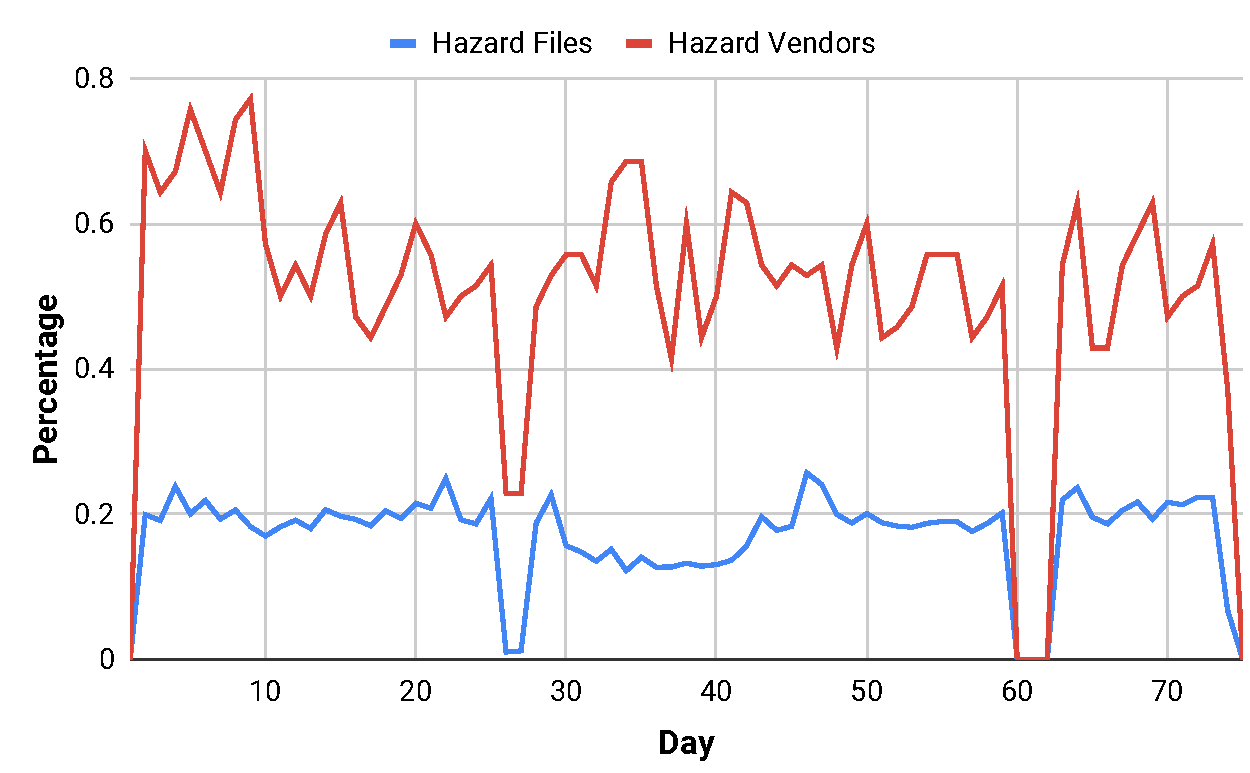
\includegraphics[width=\linewidth]{figure/hazard_day}
  \mycaption{fig:hazard_day}{How hazard flipping distribute across 75 days.}
  {}
\endminipage\hfill
\minipage{0.31\textwidth}
  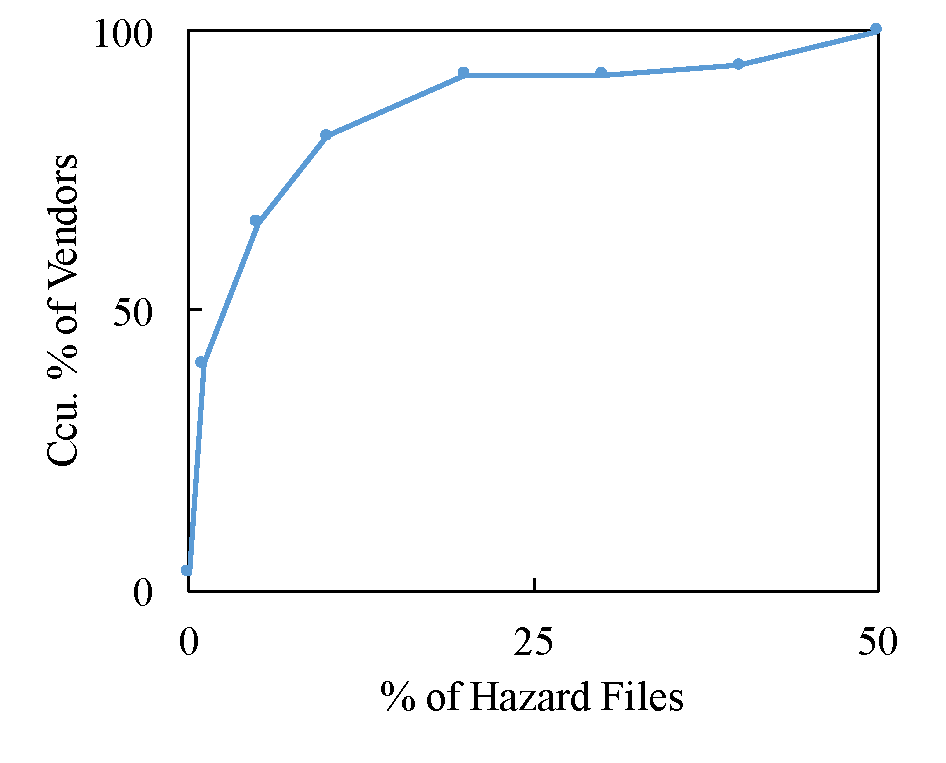
\includegraphics[width=\linewidth]{figure/hazard_vendor_file}
  \mycaption{fig:hazard_vendor_file}{Cumulative \% of vendors 
over \% of hazard files.}
  {Point (x, y) means y\% of vendors are used in less than x\% of hazard files.}
\endminipage\hfill
\minipage{0.31\textwidth}
  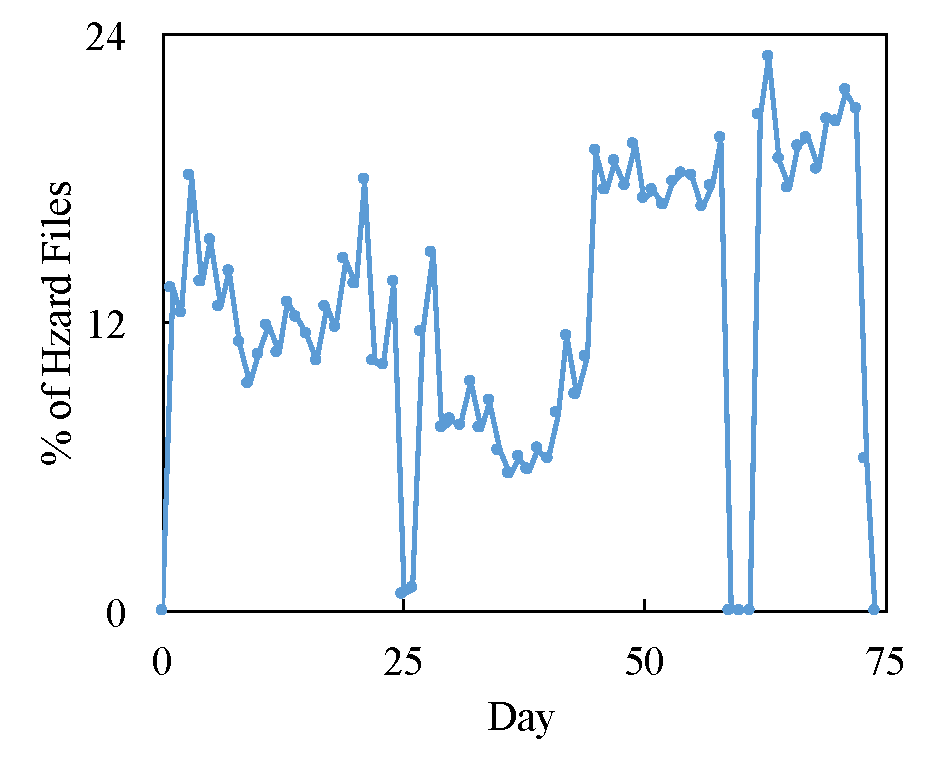
\includegraphics[width=\linewidth]{figure/hazard_day_file}
  \mycaption{fig:hazard_day_file}{ \% of hazard files for each day.}
  {}
\endminipage\hfill
\end{figure*}

\subsection{Hazard Study}

Based on our observation, some engines could continuously change their detection results when they scanned some files. We call this case as hazard flipping. In the following, we first present how hazard flipping distributes over time, and then we try to figure out reasons that could caused hazard flipping.

First, we study how hazard flipping distribute over time in our data set. Figure \ref{fig:hazard_day} present the distribution of hazard flipping across 75 days. We can see from the figure that hazard flippling widely exist in our data set. Since we missed some reports on day 60, we can not decide whether hazard flipping appears from day 59 to 61. Except for the first day and the last day, about 70 out of 75 (93.33\%) days,

\noindent{\underline{\bf{Observation 3:}}}
{\it{Hazard flipping appears almost every day in our data set, and we could not get correct results if we do not consider hazard flipping over time and only use VirusTotal with its scanning results. 
}}

An immediate question is that whether some anti-virus engines or VirusTotal API caused hazard flipping? Therefore, we then study how hazard flipping distributes over anti-virus engines and sampled files.

First, we study how many hazard files scanned by each engine. As we described in section 3, we use 64 engines to build our data set. Figure \ref{fig:hazard_vendor_file} shows how the cumulative percentage of engines changes over the percentage of hazard files. Only 2 engines have no hazard files, and we find hazard flipping from other 62 engines. Some engines could report hazard flipping results on about 50\% sampled files.

\noindent{\underline{\bf{Observation 4: }}}
{\it{More than 96.8\% anti-virus engines could report hazard flipping results when they scanned the same files for multiple times over time. Therefore, hazard flipping could not caused by misfunction of anti-virus engines. 
}}

Second, we study how the percentage of hazard files for each day. As shown in Figure \ref{fig:hazard_day_file}, not too many sampled files involve hazard flippings every day. The largest percentage is 23.08\%, and the smallest one is more than 0.6\% of 14,423 sampled files. 

\noindent{\underline{\bf{Observation 5: }}}
{\it{Although hazard flipping widely exist in anti-virus engines almost every day, we can not find all sampled files have hazard flipping per day. Hazard flipping could not caused by VirusTotal API.
}}

\begin{figure*}[!htb]
\minipage{0.31\textwidth}
  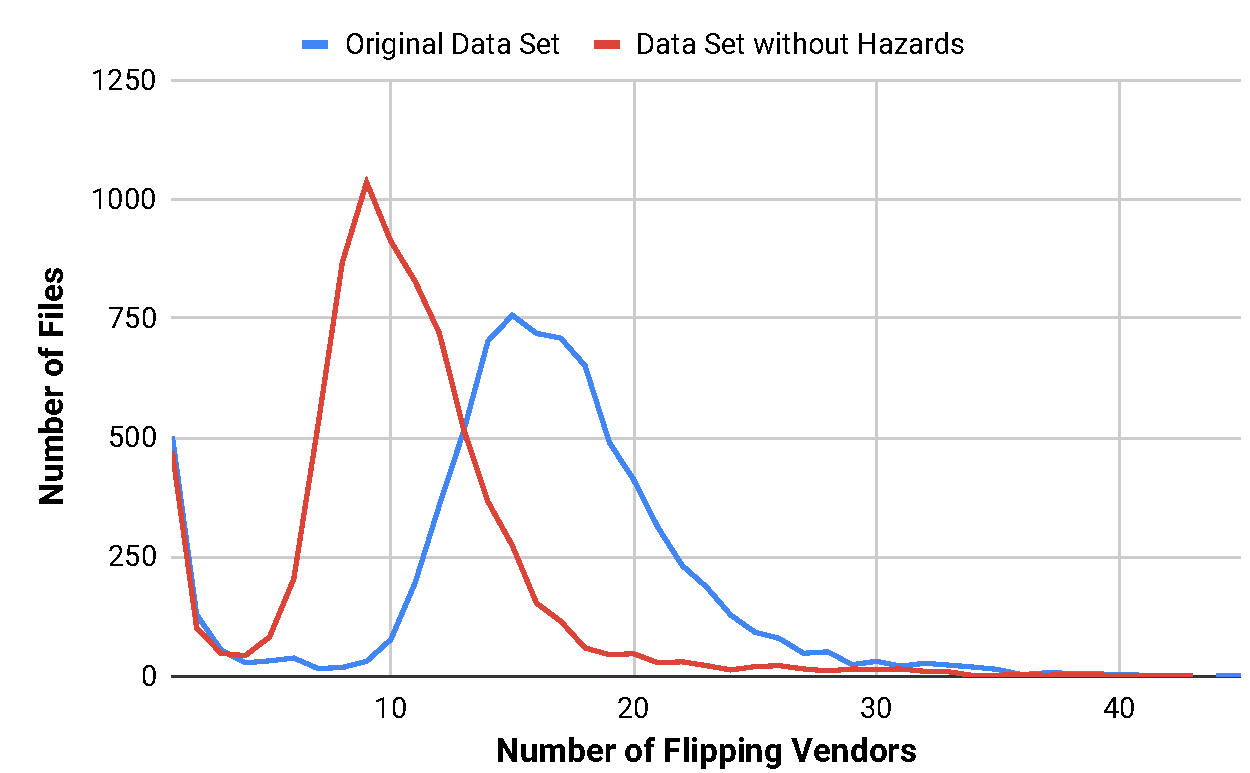
\includegraphics[width=\linewidth]{figure/flip_file}
  \mycaption{fig:flip_file}{Cumulative \% of flipping files over \# of flipping times.}
  {Point (x, y) means y\% of flipping files have less than x\# of flipping times.}
\endminipage\hfill
\minipage{0.31\textwidth}
  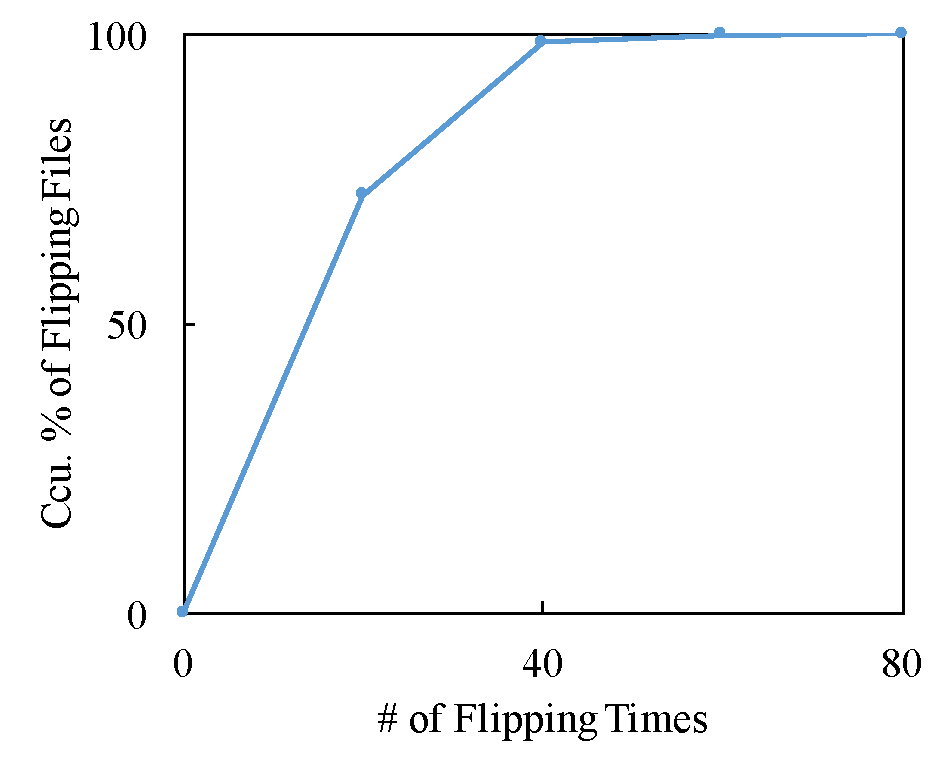
\includegraphics[width=\linewidth]{figure/flip_file_smooth}
  \mycaption{fig:flip_file_smooth}{Cumulative \% of flipping files 
over \# of flipping times.}
  {Point (x, y) means y\% of flipping files have less than x\% of flipping times.}
\endminipage\hfill
\minipage{0.31\textwidth}
  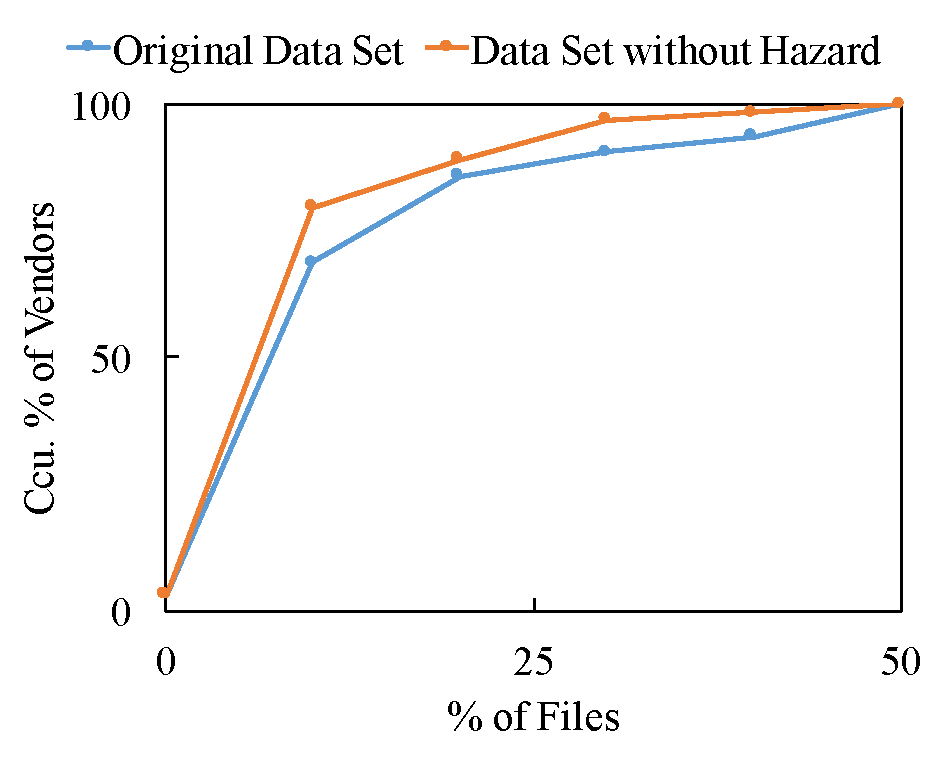
\includegraphics[width=\linewidth]{figure/flip_vendor}
  \mycaption{fig:flip_vendor}{ Cumulative \% of vendors over \% of flipping files.}
  {Point (x, y) means y\% of vendors are used in less than x\% of flipping files.}
\endminipage\hfill
\end{figure*}

\subsection{Flipping Study}

Some anti-virus engines could change their detcetion results for some random days. We call this change as flipping. In this section, we first study how flipping distributes over sampled files and engines in our data set, and then we present how result changes if we remove hazard from our data set.

In total, 7475 files have flipping results when we sumbitted 14,423 sampled files to VirusTotal for 75 days. As shown in Figure \ref{fig:flip_file}, the largest flipping times is 169, and some files flip only once in our data set. About 99.56\% flipping files have less than 120 flippings. 

\noindent{\underline{\bf{Observation 6: }}}
{\it{More than 51.8\% sampled files would have flipping detection results in our original data set. Therefore, we can not ignore the flipping of detection results when we use anti-virus engines on VirusTotal.
}}

Figure \ref{fig:flip_file_smooth} presents how flipping distributes over sampled files after removing hazards. For 7381 out of 14423 files have flipping results in our data set without hazards, and the larget flipping times 69. 

\noindent{\underline{\bf{Observation 7: }}}
{\it{Although removing hazards could reduce the flipping times of sampled files, more than 51.1\% of files have flipping results. 
}}
%Figure y presents the cumulative percentage of flipping files over the number of engines. For a sampled file, at most 39 engines would change their detection results during 75 days. About 99.5\% flipping files involve less than 30 engines in our data set. 

%Obeservation 7: For a file, at most 60.9\% engines would change their detection results over time. 

Figure \ref{fig:flip_vendor} shows how the cumulative percentage of engines over the percentage of sampled files. More than 96.8\% anti-virus engines have flipping detection results, and only 2 engines report no flipping results during 75 days in our data set. For each engine, it would change their detection results on at most 43.34\% sampled files. When we removed hazards from our data set, there are still 62 vendors could change their detection results.

\noindent{\underline{\bf{Observation 8: }}}
{\it{Most anti-virus engines could change detection results with flipping. For each engine, it could change its detection result on some sampled files. We should consider flipping results from engines when we use VirusTotal.
}}


%Todo: add hazard discussion in this part before discussing flipping. 

%Hazard caused by VT API? NO

%Hazard caused by vendor misfunction? NO

%conclusion: randomly appear, but quite frequently, affect lots of files

%Conclusion: remove hazard before studying flipping?

%Run experiments both with and without hazard
%\textbf{Summary:} Hazard pattern is obviously common in our results and it affects lots of files and vendors. An immediate question that follows is what our results would be if we remove hazards before studying the flipping pattern? We will give more explanations of our experiments in the following sections.  


%\textbf{Summary:} Flipping pattern widely exists in our experiments. Statistically, more than 50\% files and 97\% vendors have flipping patterns. Removing hazards is an effective approach to reduce flipping patterns for some vendors, but only 97 files have no flipping pattern after smoothing hazards. A large numbers of files and vendors still have flipping patterns. Flipping pattern is the most important reason that results in many files and vendors to be unstable.


\subsection{Conclusions}
